\NeedsTeXFormat{LaTeX2e}[1995/12/01]
\documentclass[10pt]{bmc_article}


% Load packages
%\usepackage{hyperref}
\usepackage{cite} % Make references as [1-4], not [1,2,3,4]
\usepackage{url} % Formatting web addresses
\usepackage{ifthen} % Conditional
\usepackage{multicol} %Columns
\usepackage{xspace}
\usepackage[utf8]{inputenc} %unicode support
%\usepackage[applemac]{inputenc} %applemac support if unicode package fails
%\usepackage[latin1]{inputenc} %UNIX support if unicode package fails
\urlstyle{rm}
\usepackage[OT1]{fontenc} 

\usepackage{rotating}
\usepackage{colortbl}
\usepackage{color}
\usepackage{comment}

\usepackage{subfigure}

\newcommand {\pg}[1]{\textcolor{blue}{#1}}
\newcommand {\ppg}[1]{\textcolor{blue}{#1}}
\newcommand {\new}[1]{\textcolor{green}{#1}}

\newcommand{\minitab}[2][l]{\begin{tabular}{#1}#2\end{tabular}}


%\newcommand{} {\mbox{}\xspace}

\def\squeezetable{\def\tabular@font{\tiny}}%

% Change useable area of a page to be slightly larger
\setlength{\topmargin}{0.0cm}
\setlength{\textheight}{21.5cm}
\setlength{\oddsidemargin}{0cm}
\setlength{\textwidth}{16.5cm}
\setlength{\columnsep}{0.6cm}

\newboolean{publ}

%Settings: comment\uncomment bmcformat definition to get format required

%Review style settings
\newenvironment{bmcformat}{\begin{raggedright}\baselineskip20pt\sloppy\setboolean{publ}{false}}{\end{raggedright}\baselineskip20pt\sloppy}

%Publication style settings
%\newenvironment{bmcformat}{\fussy\setboolean{publ}{true}}{\fussy}


% Begin ...
\begin{document}
\begin{bmcformat}

%\title{Non-coding RNAs of bird genomes}
%\title{Wins and losses: Non-coding RNAs of bird genomes}
\title{Fly away Peter, come back Paul: the conservation and losses of avian non-coding RNAs}

\author{
Paul P.\ Gardner\correspondingauthor$^{1,2}$
\email{Paul P.\ Gardner\correspondingauthor - paul.gardner@canterbury.ac.nz},
Jana Hertel$^5$
\email{Jana Hertel\correspondingauthor - jana@bioinf.uni-leipzig.de},
Sarah W.\ Burge$^3$
\email{swb@ebi.ac.uk},
Maria Ninova$^4$
\email{Maria.Ninova@postgrad.manchester.ac.uk},
Stephanie Kehr$^5$
\email{steffi@bierdepot.bioinf.uni-leipzig.de},
Mario Fasold$^5$
\email{mario@bierdepot.bioinf.uni-leipzig.de},
Tammy E.\ Steeves$^1$
\email{tammy.steeves@canterbury.ac.nz},
Sam Griffiths-Jones$^4$
\email{sam.griffiths-jones@manchester.ac.uk}
and
Peter F.\ Stadler\correspondingauthor$^5$
\email{Peter Stadler\correspondingauthor - studla@bioinf.uni-leipzig.de}
}
\address{
\iid(1) School of Biological Sciences, University of Canterbury, Private Bag 4800, Christchurch, New Zealand.
\iid(2) Biomolecular Interaction Centre, University of Canterbury, Private Bag 4800, Christchurch, New Zealand.
\iid(3) European Molecular Biology Laboratory, European Bioinformatics Institute, Hinxton, Cambridge, CB10 1SD, UK.
\iid(4) Faculty of Life Sciences, University of Manchester, Manchester, United Kingdom.
\iid(5) Bioinformatics Group, Department of Computer Science; and Interdisciplinary Center for Bioinformatics, University of Leipzig, H{\"a}rtelstrasse 16-18, D-04107 Leipzig, Germany
}

\maketitle

\begin{abstract}
Here we present the results of a large-scale bioinformatic annotation
of non-coding RNAs in 48 avian genomes. Our approach uses
probabilistic models of hand-curated families from the Rfam database
to infer conserved RNA families within each avian genome. We
supplement these annotations with predictions from the tRNA annotation
tool, tRNAscan-SE and microRNAs from miRBase.  We show a significant
number of lncRNAs are surprisingly well conserved between birds and
mammals including several intriguing cases where the reported
mammalian lncRNA function is not conserved in birds.  We also
demonstrate extensive conservation of classical ncRNAs (e.g., tRNAs)
and more recently discovered ncRNAs (e.g., snoRNAs and miRNAs) in
birds. Furthermore, we have discovered apparent ``losses'' in several
RNA families, these include the divergence of some classical ncRNAs
and the loss of several snoRNAs and microRNAs.  These combined results
illustrate the utility of applying homology based methods for
annotating vertebrate genomes and illustrate many complex evolutionary
patterns within the avian ncRNA cohort.
\end{abstract}

%% Non-coding RNAs in bird genomes

%% Paul P. Gardner1,2, Sarah W. Burge3, Jana Hertel5, Maria Ninova4, Stephanie Kehr5, Anne Nitsche5, Mario Fasold5, Tammy E. Steeves1, Sam Griffiths-Jones4, Peter Stadler5

%% 1 School of Biological Sciences, University of Canterbury, Private Bag 4800, Christchurch, New Zealand. 2 Biomolecular Interaction Centre, University of Canterbury, Private Bag 4800, Christchurch, New Zealand. 3 European Molecular Biology Laboratory, European Bioinformatics Institute, Hinxton, Cambridge, CB10 1SD, UK. 4Faculty of Life Sciences, University of Manchester, Manchester, United Kingdom. 5 Bioinformatics Group, Department of Computer Science; and Interdisciplinary Center for Bioinformatics, University of Leipzig, Hartelstrasse 16-18, D-04107 Leipzig, Germany
 
%% Talking points:
%% 1. Although the majority of classical eukaryotic ncRNAs are conserved in birds, several notable classical ncRNAs are not. Homology searches in associated genes indicate these apparent "losses" are most likely due to divergence.
%% 2. Of the 59 snoRNA conserved between humans and yeast, we find 45 are conserved in birds. Homology searches in associated genes for the remaining non-conserved snoRNAs indicate these apparent losses are indeed due to multiple losses in several bird lineages.
%% 3. We find that 3 families of broadly conserved vertebrate microRNA families are lost in the avian lineage. We also annotate a number of bird-specific microRNAs.
%% 4. Several well-characterised lncRNA families of known function are conserved between mammals and birds.
%% 5. We discuss the conservation of HOX associated lncRNAs and several lncRNAs that have been implicated in processes associated with cancer.
 
%% %% Draft Abstract
%% We present the results of a large-scale bioinformatic annotation of non-coding RNAs in 48 avian genomes. We use probabilistic models of hand-curated families from the Rfam database to infer conserved RNA families within each avian genome. We supplement these annotations with predictions from the tRNA annotation tool, tRNAscan-SE, microRNAs from miRBase and selected sequences from analyses of the chicken transcriptome. Although we show extensive conservation of classical ncRNAs (e.g., tRNAs and rRNAs) and more recently discovered ncRNAs (e.g., snoRNAs and miRNAs) in birds, we also demonstrate apparent ``losses'' in several RNA families. These include the divergence of some classical ncRNAs and the genuine loss of several snoRNAs and microRNAs. In contrast, we show a signicant number of lncRNAs are surprisingly well conserved between birds and mammals including several intriguing cases where the reported mammalian lncRNA function is not conserved in birds. These combined results illustrate the utility of applying homology based methods for annotating vertebrate genomes and illustrate many complex evolutionary patterns within the avian ncRNA cohort.

%% LNCRNA:


\ifthenelse{\boolean{publ}}{\begin{multicols}{2}}{}

\section*{Introduction}

Non-coding RNAs (ncRNAs) are an important class of genes, responsible
for the regulation of many key cellular functions. The major RNA
families include the classical, highly conserved RNAs, sometimes
called ``molecular fossils'', such as the transfer RNAs, ribosomal
RNAs, RNA components of RNase P and the signal recognition particle
\cite{Jeffares:1998}. Other classes appear to have have evolved more
recently, e.g. the small nucleolar RNAs (snoRNAs), microRNAs (miRNAs)
and the long non-coding RNAs (lncRNAs) \cite{Hoeppner:2012}.

The ncRNAs pose serious research challenges, particularly for the
field of genomics. For example, they lack the strong statistical
signals associated with protein coding genes, e.g. open reading
frames, G+C content and codon-usage biases \cite{Rivas:2000}. Despite
promising techniques such as RNA-seq \cite{Croucher:2010}, homology
based methods, namely covariance models (CMs) remain state of the art
for ncRNA analyses \cite{Sakakibara:1994,Eddy:1994,Nawrocki:2009}.
The CM based approach for annotating ncRNAs in genomes requires
reliable alignments and consensus secondary structures of
representative sequences of RNA families. These are used to train
probabilistic models for each family. These models can be used to
generate sequences with similar properties, score the likelihood that
a sequence is generated by the same evolutionary processes as the
training sequences and to build alignments based upon sequence and
structural information \cite{Sakakibara:1994,Eddy:1994,Nawrocki:2009}.
The tRNAscan-SE software package uses CMs to accurately predict
transfer RNAs \cite{Lowe:1997,Chan:2009}.  The Rfam database contains
thousands of curated alignments and consensus structures for diverse
classes of ncRNAs
\cite{Griffiths-Jones:2003,Griffiths-Jones:2005,Gardner:2009,Gardner:2011a,Burge:2013}.
Independent benchmarks of bioinformatic annotation tools have shown
that the CM approaches dramatically out-perform alternative methods
\cite{Freyhult:2007}, although its sensitivity is limited for the most
rapidly evolving families such as vault RNAs or telomerase RNA
\cite{Menzel:09a}.

The CM based approach works well for almost all classes of ncRNA, but
the long non-coding RNAs (lncRNAs) are a particular challenge
\cite{Guttman:2009}. Recent technological advances have led to
dramatic speed and memory-usage enhancements for CM analyses
\cite{Eddy:2002,Nawrocki:2007,Nawrocki:2009,Eddy:2011}. However, CMs
cannot model the exon-intron structures of spliced lncRNAs, nor can
they deal simply with the repeats that many lncRNAs host. Consequently
in the latest release of Rfam the lncRNA families that were added were
composed of local conserved (and possibly structured elements) within
lncRNAs, analogous to the ``domains'' housed within protein sequences
\cite{Burge:2013}. The functions determined to date for lncRNAs range
from regulating chromatin status to chromosomal inactivation
\cite{Rinn:2007,Chow:2005}. Yet functional characterisation of these
genes is a lengthy and expensive process \cite{Guttman:2009}.

The publication of 48 avian genomes, including the previously
published chicken
\cite{International_Chicken_Genome_Sequencing_Consortium:2004}, zebra
finch \cite{Warren:2010} and turkey \cite{Dalloul:2010} with the newly
published 45 avian genomes \cite{birds:14,birds:14a}, provides
exciting opportunities to to explore ncRNA conservation in
unprecedented detail.

In the following we explore the conservation patterns of the major
classes of avian ncRNA in further detail. The collection of ncRNA
sequences is generally biased towards model organisms
\cite{Gardner:2010,Hoeppner:2012}. We focus our report on the unusual
results within the avian lineages. These are either unexpectedly
well-conserved RNAs or unexpectedly poorly-conserved RNAs. The former
are RNAs we would not have expected to be conserved between the birds
and the organisms these genes were initially identified in; Usually,
this hypothesis is based upon the function of the RNA which is not
conserved in avian species. The latter are apparent losses of RNA
genes that were expected to be conserved; usually, this hypothesis is
based upon the conservation of these RNAs in other vertebrate species.
We use three models of ``loss'' that explain the data: Firstly, these
could be genuine cases of an ancestral gene-loss along the avian
lineage. Secondly, this could be a case of ``divergence'' where a RNA
gene has undergone significant sequence and structural alterations, so
much so, that our homology search tools can no longer detect a
relationship between vertebrate exemplars and the avian
varieties. Thirdly, we consider the possibility that the available
genome assemblies have independently failed to capture these genes.

\section*{Results}


\subsection*{Unusually well conserved RNAs}

The bulk of the ``unusually well conserved RNAs'' belong to the long
non-coding RNA (lncRNA) group.  The lncRNAs are a diverse group of
RNAs that have been implicated in a multitude of functional processes
\cite{Rinn:2007,Chow:2005,Guttman:2009}. These RNAs have largely been
characterised in mammalian species, particularly human and
mouse. Consequently, we generally do not expect these to be conserved
outside of mammalia. Notable examples include Xist \cite{Duret:2006}
and H19 \cite{Smits:2008}.  There is emerging evidence for the
conservation of ``mammalian'' lncRNAs in other vertebrates
\cite{Chodroff:2010,Ulitsky:2011}), however, like most lncRNAs, the
function of these lncRNAs remains largely unknown. Here, we show the
conservation of several well-characterised lncRNAs of known function
in humans. 

In general, Rfam cannot include the entire length of any large, spliced
RNAs. This is a limitation of the covariance-models used for the
homology-searches Rfam runs \cite{Nawrocki:2009}. Consequently, only
short, well-conserved regions with evolutionarily conserved secondary
structures are included in Rfam. By analogy to protein-domains, we
refer to these as RNA-domains \cite{Burge:2013}.

When analysing the RNA-domain annotations it is striking that many of
the lncRNAs with multiple RNA-domains are consistently preserved in
the birds. The annotations of these domains lie in the same genomic
region, in the same order as in the mammalian homologs. Thus they
support a high degree of evolutionary conservation for the entire
lncRNA. In particular the HOXA11-AS1, PART1, PCA3, RMST, Six3os1, SOX2OT and
ST7-OT3 lncRNAs have multiple, well conserved RNA-domains (See
Figure~\ref{fig:5}).

The conservation of these ``human'' lncRNAs among birds suggests they may 
also be functional in birds but what these
functions is not immediately obvious. For example, PART1 and
PCA3 are both described as prostate-specific lncRNAs that play a role
in the human androgen-receptor pathway
\cite{Bussemakers:1999,Lin:2000,Ferreira:2012}. Birds lack a prostate
but both males and females express the androgen receptor (AR or NR3C4) in gonadal
and non- gonadal tissue
\cite{Yoshimura:1993,Veney:2004,Fuxjager:2012,Leska:2012}. Thus, we
postulate that PART1 and PCA3 also play a role in the
androgen-receptor pathway in birds but whether the expression of these
lncRNAs are tissue specific is unknown at present.

The HOX cluster lncRNAs HOTAIRM1 (5 RNA-domains), HOXA11-AS1 (6
RNA-domains), and HOTTIP (4 RNA domains) are remarkably well conserved. In
the human genome they are located in the HOXA cluster (hg coordinates
chr7:27135743-27245922), one of the most highly conserved regions in
vertebrate genomes \cite{PascualAnaya:13}, in antisense orientation between
HoxA1 and HoxA2, between HoxA11 and HoxA13, and upstream of HoxA13,
respectively. Conservation and expression of HOTAIRM1 and HOXA11-AS1 within
the HOXA cluster has been studied in some detail in marsupials
\cite{Yu:12}.  Of the 15 RNA-domains five and six representing all three
lncRNAs were recovered in the alligator and turtle genomes. All of them
appear in the correct order at the expected, syntenically conserved
positions within the HOXA cluster.  In the birds, where two or more of the
HOX cluster lncRNA RNA-domains were predicted on the same scaffold, this
gene order and location within HOX was also preserved.

%egrep 'HOXA11-AS1|HOTAIR|HOTTIP' clans_competed/*gff | perl -lane 'if(/\/(\S+?)\-.*gff:(\S+).*\-id=(\S+);eval/ or /\/(\S+?)\-.*gff:(\S+).*Alias=(\S+);Not/){print "$1\t$2\t$3\t$F[6]"}'
%egrep 'PCA3' clans_competed/*gff | perl -lane 'if(/\/(\S+?)\-.*gff:(\S+).*\-id=(\S+);eval/ or /\/(\S+?)\-.*gff:(\S+).*Alias=(\S+);Not/){print "$1\t$2\t$3\t$F[6]"}'
%egrep 'RMST' clans_competed/*gff | perl -lane 'if(/\/(\S+?)\-.*gff:(\S+).*\-id=(\S+);eval/ or /\/(\S+?)\-.*gff:(\S+).*Alias=(\S+);Not/){print "$1\t$2\t$3\t$F[6]"}'

Many of the lncRNAs have been associated with cancer, sparking a minor
review industry \cite{Prensner:2011,Spizzo:2012}. Three examples of
these that are also conserved in the birds are described below.

The RMST (Rhabdomyosarcoma 2 associated transcript) RNA-domains 6, 7,
8, and 9 are conserved across the birds. In each bird the gene order
was also consistent with the human ordering. In the alligator and
turtle an additional RNA-domain was predicted in each, these were
RNA-domains 2 and 4 respectively, again the ordering of the domains
was consistent with human. This suggests that the RMST lncRNA is
highly conserved. However, little is known about the function of this
RNA. It was originally identified in a screen for differentially
expressed genes in two Rhabdomyosarcoma tumor types \cite{Chan:2002}.

In addition, the lncRNA DLEU2 is well conserved across the
vertebrates, it is a host gene for two miRNA genes, miR-15 and miR-16,
both of which are also well conserved across the vertebrates (See
Supplemental Figure~2). DLEU2 is thought to be a tumor-suppressor gene
as it is frequently deleted in malignant tumours
\cite{Lerner:2009,Klein:2010}.

The NBR2 lncRNA and BRCA1 gene share a bidirectional promotor
\cite{Xu:1997}. Both are expressed in a broad ranch of
tissues. Extensive research on BRCA1 has shown that it is involved in
DNA repair \cite{Moynahan:1999}. The function of NBR2 remains unknown,
yet its conservation across the vertebrates certainly implies a
function (See Figure~\ref{fig:5}).

Of the other classes of RNAs, none showed an unexpected degree of
conservation or expansion within the avian lineage. The only exception
being the snoRNA SNORD93 which we show has 92 copies in the tinamou
genome, whereas it only has 1-2 copies in all the other vertebrate
genomes. 

\subsection*{RNA Losses, divergence or missing data?}

Much of the number of apparent losses and reduction in genomic
sequence has been extensively discussed elsewhere
\cite{Organ:2007}. Unsurprisingly, this reduction is reflected in the
copy-number of RNA genes. Some of the most dramatic examples are the
transfer RNAs and pseudogenes which average $\approx 900$ and $\approx
580$ copies in the human, turtle and alligator genomes, the average
copies numbers of these drop to $\approx 280$ and $\approx 100$ copies
in the avian genomes. 

The absence of several well-conserved ncRNA families from many or even most
bird genomes is unlikely to represent true gene losses. This concerns in
particular the telomerase RNA, the RNA components of RNase P and MRP, the
minor spliceosomal snRNAs U4atac and U11, the selenocystein tRNA (tRNA-Sec)
as well as the vault RNAs. In order to get an idea to what extent the
absence of these RNAs from the \texttt{infernal-based} annotation is caused 
by sequence divergence beyond the thresholds of the Rfam CMs and/or 
missing or incomplete data, we complemented our analysis by dedicated
searches for a few of these RNA groups. 

The simplest case are the selenocystein tRNAs. Here, tRNAscan is tuned
for specificity and thus misses several occurrances that are easily
found by \texttt{blastn} with $E\le 10^{-30}$. In some cases the
sequences appear degraded at the ends, which may be explained e.g.\ by
low sequence quality at the very ends of contigs or scaffolds. A
\texttt{blastn} search also readily retrieves additional RNAse P and
RNAse MRP RNAs, capturing only the best conserved regions. In many
cases these additional candidates are incomplete or contain
undetermined sequence, explaining why they are missed by the
CMs. Overall, we identify tRNA-Sec in most and RNAse P and MRP RNAs in
the majority of the genomes. An additional candidate could also be
retrieved for telomerase RNA. Telomerase is well known to exhibit very
poor sequence conservation and rapid variations in size that make it
notoriously hard to identify by homology search \cite{Xie:08a}. The
poor return thus does not come as a surprise. Since \texttt{blastn}
searches remained unsuccessfull we constructed a sauropsid-specific CM
for the vault RNA. In addition to the hits identified by the Rfam
model we obtained three additional homologs. Vault RNAs, with a size
of about 100 nt, exhibit conserved sequence patterns only at their
ends, with essentially unconstrained sequence in the central
part. Their identification is one of the well-know difficult problems
for homology search \cite{Stadler:09b}.

Our ability to find additional homologs for several RNA families that fill
gaps in the abundance matrices (Figure~\ref{fig:7})
strongly suggests that conspicuous absences, in particular of LUCA and
LECA RNAs, are caused by incomplete data in the current assemblies and
sequence divergence rather then true losses.

%\subsection*{Y RNA clusters} 

Vertebrate Y RNAs typically form a cluster comprising four
well-defined paralog groups Y1, Y3, Y4, and Y5. In line with
\cite{Mosig:07a} we find that the Y5 paralog family is absent from all
bird genomes, while it is still present in both alligator and turtle,
see Supplemental Figure~4. Within bird, we find an the conserved
Y4-Y3-Y1 cluster. Apparently, broken-up clusters are in most cases
consistent with breaks in the available sequence assemblies. In
several genomes we observe one or a few additional Y RNA homologs
unlinked to the canonical Y RNA cluster. These sequences can be
identified unambiguously as derived members of one of the three
ancestral paralog groups, they almost always fit less well to the
consensus (as measured by the CM bit score of paralog group specific
covariance models) than the paralog linked to cluster, and there is no
indication that any of these additional copies is evolutionarily
conserved over longer time scales. We therefore suggest that most or
all of these interspersed copies are in fact pseudogenes.

%\subsection*{MicroRNA clusters} 

Nearly all microRNAs that are broadly conserved in fish, amphibians and
mammals are also conserved in the birds. Nevertheless, there are obvious
instances of microRNAs lost in all birds. For example, mammalian and
ambhibian genomes contain three loci of clustered microRNAs from the mir-17
and mir-92 families \cite{Tanzer:04}. One of these clusters (cluster II,
with families mir-106b, mir-93 and mir-25) was not found in turtles,
crocodiles and birds, see Supplemental Figure~6.

The microRNA family let-7 is the most diverse microRNA family with 14
paralogs in human. These genes also localize in 7 genomic clusters,
together with mir-100 and mir-125 miRNA families (see previous study on the
evolution of the let-7 miRNA cluster in \cite{Hertel:2012}). In Sauropsids
we observed that cluster A - which is strongly conserved in vertebrates has
been completely lost in the avian lineage. Another obvious loss in birds is
cluster F, containing two let-7 microRNA paralogs. Cluster H, on the other
hand has been retained in all oviparous animals and completely lost later,
after the split of Theria. See Supplemental Figure~7 for details.

\section*{Conclusions}

%Talking points:
%1. several classical RNAs (e.g. spliceosomal, telomerase, RNase MRP
%RNAs) have diversified in birds relative to other Eukaryotes.
%2. several lncRNA families are conserved between mammals and
%birds. Several of these are characterised by expression in tissues
%that are not present in birds (e.g. the prostate).
%3. several regulatory RNAs, snoRNAs and microRNAs, have been lost
%since the birds diverged from the other vertebrates. Indicating many
%avian-specific alterations in gene regulation.

In this work we have provided a comprehensive annotation of non-coding
RNAs in genome sequences using homology-based methods. The
homology-based tools have distinct advantages over experimental-based
approaches as not all RNAs are expressed in any particular tissue-type
or developmental-stage, in fact some RNAs have extremely specific
expression profiles \cite{Johnston:2003}.  We have identified
previously unrecognised conservation of ncRNAs in avian genomes as
well as some surprising ``losses'' of otherwise well conserved
ncRNAs. We suspect many of these losses are due to a combination of
limitations in the homology search tools that we use for annotation
and the ability of ncRNAs to tolerate large amounts of sequence
variation while remaining functional, rather than \emph{bona fide}
gene loss. In some cases these losses could be due to missing data
from the genome assemblies, but this unlikely to be the case for
multiple independant assemblies.

These results indicate we are still in the very early phases of
determining the functions of many RNA families. This is illustrated by
the fact that the reported functions of some ncRNAs are
mammal-specific, yet some are also found in bird genomes. CITE DAVE
BURT ET AL AND THE COMPARATIVE ARTICLE?

\section*{Methods}

Bird genomes were searched using the cmsearch program from INFERNAL
1.1 and the covariance models from the Rfam database
v11.0 \cite{Gardner:2011a,Burge:2013}. All matches above the curated GA
threshold were included. Subsequently, all hits with an E-value
greater than 0.0005 were discarded, so only matches which passed the
model-specific GA threshold and had an E-value smaller than 0.0005
were retained. The Rfam database classifies non-coding RNAs into
hierarchial groupings. The basic units are ``families'' which are
groups of homologous, alignable sequences; ``clans'' which are groups
of un-alignable (or functionally distinct), homologous families; and
``classes'' which are groups of clans and families with related
biological functions e.g. spliceosomal RNAs, miRNAs and snoRNAs
\cite{Griffiths-Jones:2003,Griffiths-Jones:2005,Gardner:2009,Gardner:2011a,Burge:2013};
these categories have been used to classify our results.

In order to obtain good annotations of tRNA genes we also ran the
specialist tRNA-scan version 1.3.1 annotation tool. This method also
uses covariance models to identify tRNAs. However it also uses some
heuristics to increase the search-speed, annotates the Isoacceptor
Type of each prediction and uses sequence analysis to infer if
predictions are likely to be functional or tRNA-derived pseudogenes
\cite{Lowe:1997,Chan:2009}.

Rfam matches and the tRNA-scan results for families belonging to the
same clan were then ``competed'' so that only the best match was
retained for any genomic region \cite{Gardner:2011a}.  To further
increase the specificity of our annotations we filtered out families
that were indentified in four or fewer of the 51 vertebrate species we
have analysed in this work. These filtered families largely
corresponded to bacterial contamination within the genomic sequences.

999 microRNA sequence families, previously annotated in at least one
vertebrate, were retrieved from miRBase (v19). Individual sequences or
multiple sequence alignments were used to build covariance models with
INFERNAL (v1.1rc3), and these models were searched against the 48 bird
genomes, and the genomes of the american alligator and the green
turtle as outgroups. Hits with e-value <10 realigned with the query
sequences and the resultant multiple sequence alignments manually
inspected and edited using RALEE.

An additonal snoRNA homology search was performed with snoStrip
\cite{Bartschat:2013}. As initial queries we used deutorostomian
snoRNA families from human \cite{Lestrade:2006}, platypus
\cite{Schmitz:2008}, and chicken \cite{Shao:2009}.

%SnoRNA annotations overlapping miRNAs annotations where manually
%inspected \ppg{and?...}.



Chicken snoRNA and miRNA annotations were validated using small
RNA-seq data comprising 27 samples from 14 diferent tissues. Since not
all RNAs are expressed at any given time we expect to verify only a
fraction of annotated RNAs using the expression data. Nevertheless 242
of 691 (35\%) miRNAs as well as 328 of 376 (87\%) snoRNAs of our
homology-based annotations were found to be supported by the RNA-seq
data.


\section*{Acknowledgements}

Erich Jarvis (Duke University), Guojie Zhang (BGI-Shenzhen \&
University of Copenhagen) and Tom Gilbert (University of Copenhagen)
for access to data and for invaluable feedback on the manuscript.

Magnus Alm Rosenblad (Univ. of Gothenburg) for useful discussions.

We thank Fiona McCarthy (Mississippi State University) and Carl
Schmidt (University of Delaware) for providing the RNA-seq data.

%%%%%%%%%%%%%%%%%%%%%%
%% The Bibliography %%
%%
%% ---------------------------------
%% BioMedCentral bibtex .BST file will be used to
%% create a .BBL file which includes the BMC XML.
%% Note that the displayed Bibliography will not be
%% exactly as specified in the online Instructions for Authors


{\ifthenelse{\boolean{publ}}{\footnotesize}{\small}
\bibliographystyle{bmc_article} % Style BST file
 \bibliography{bird} } % Bibliography file (usually '*.bib' )

%%%%%%%%%%%

\clearpage
\newpage


\begin{figure}[ht]
  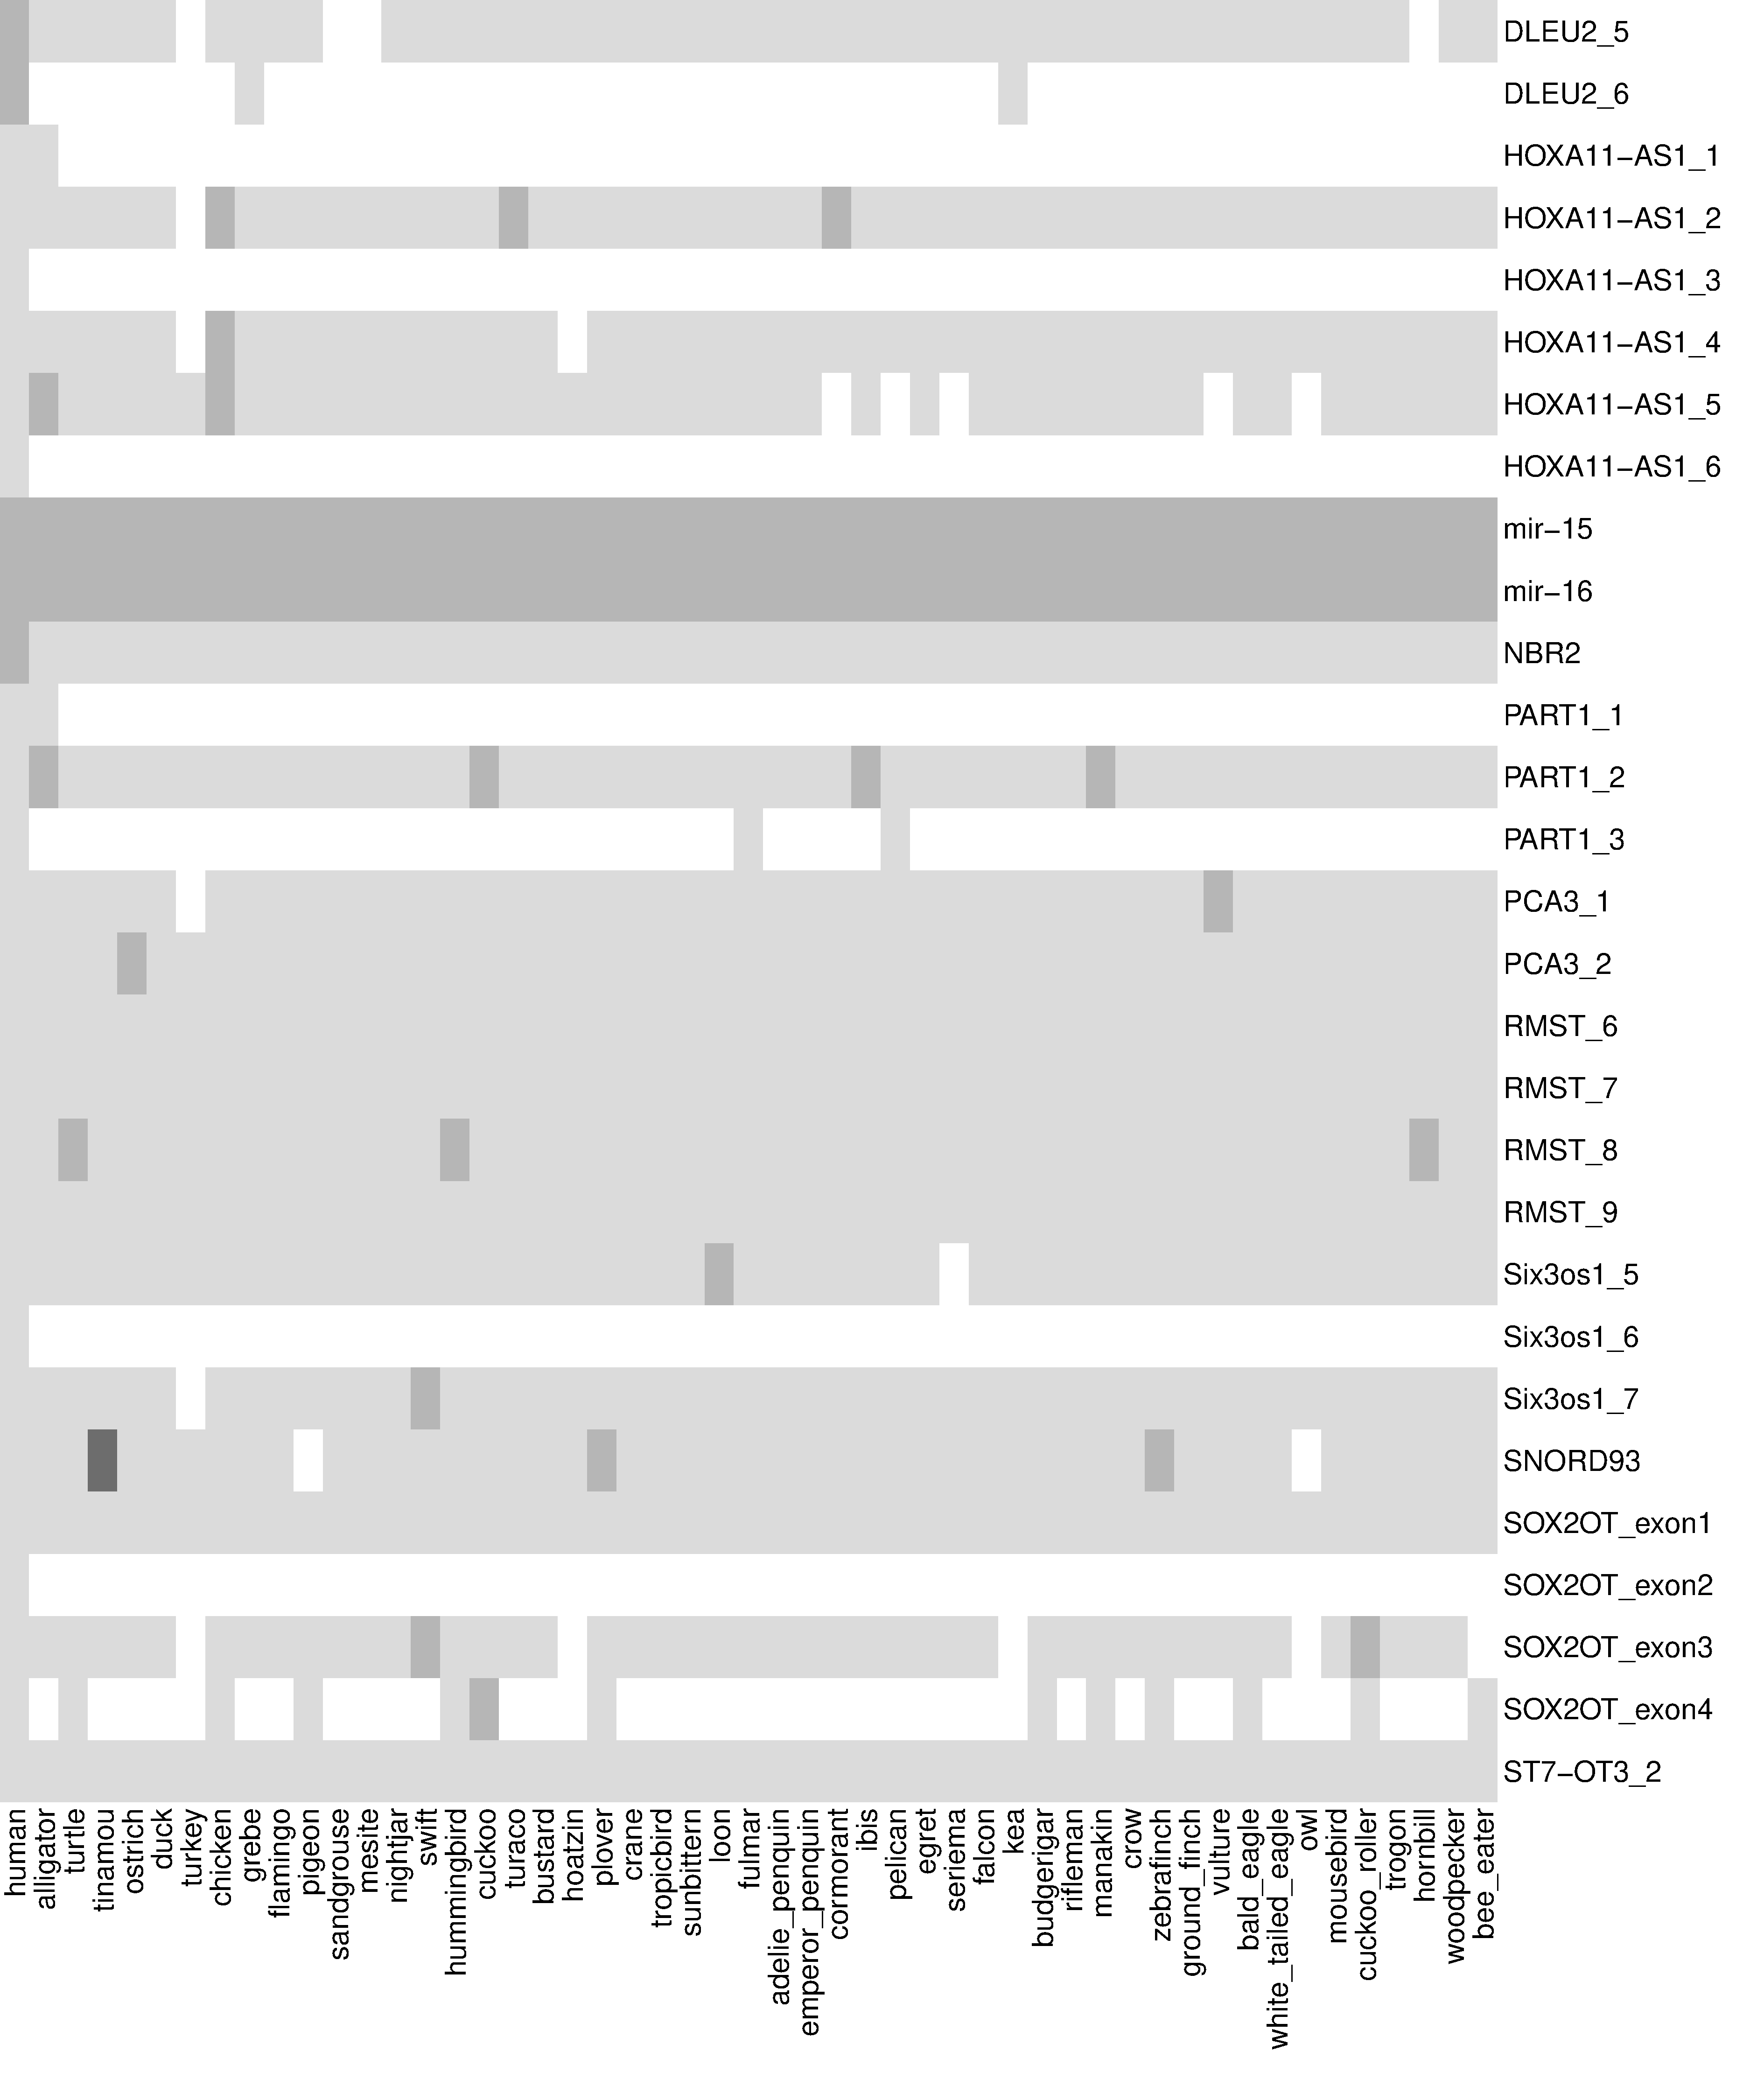
\includegraphics[width=0.45\textwidth]{figures/unusual-conserved.pdf}
  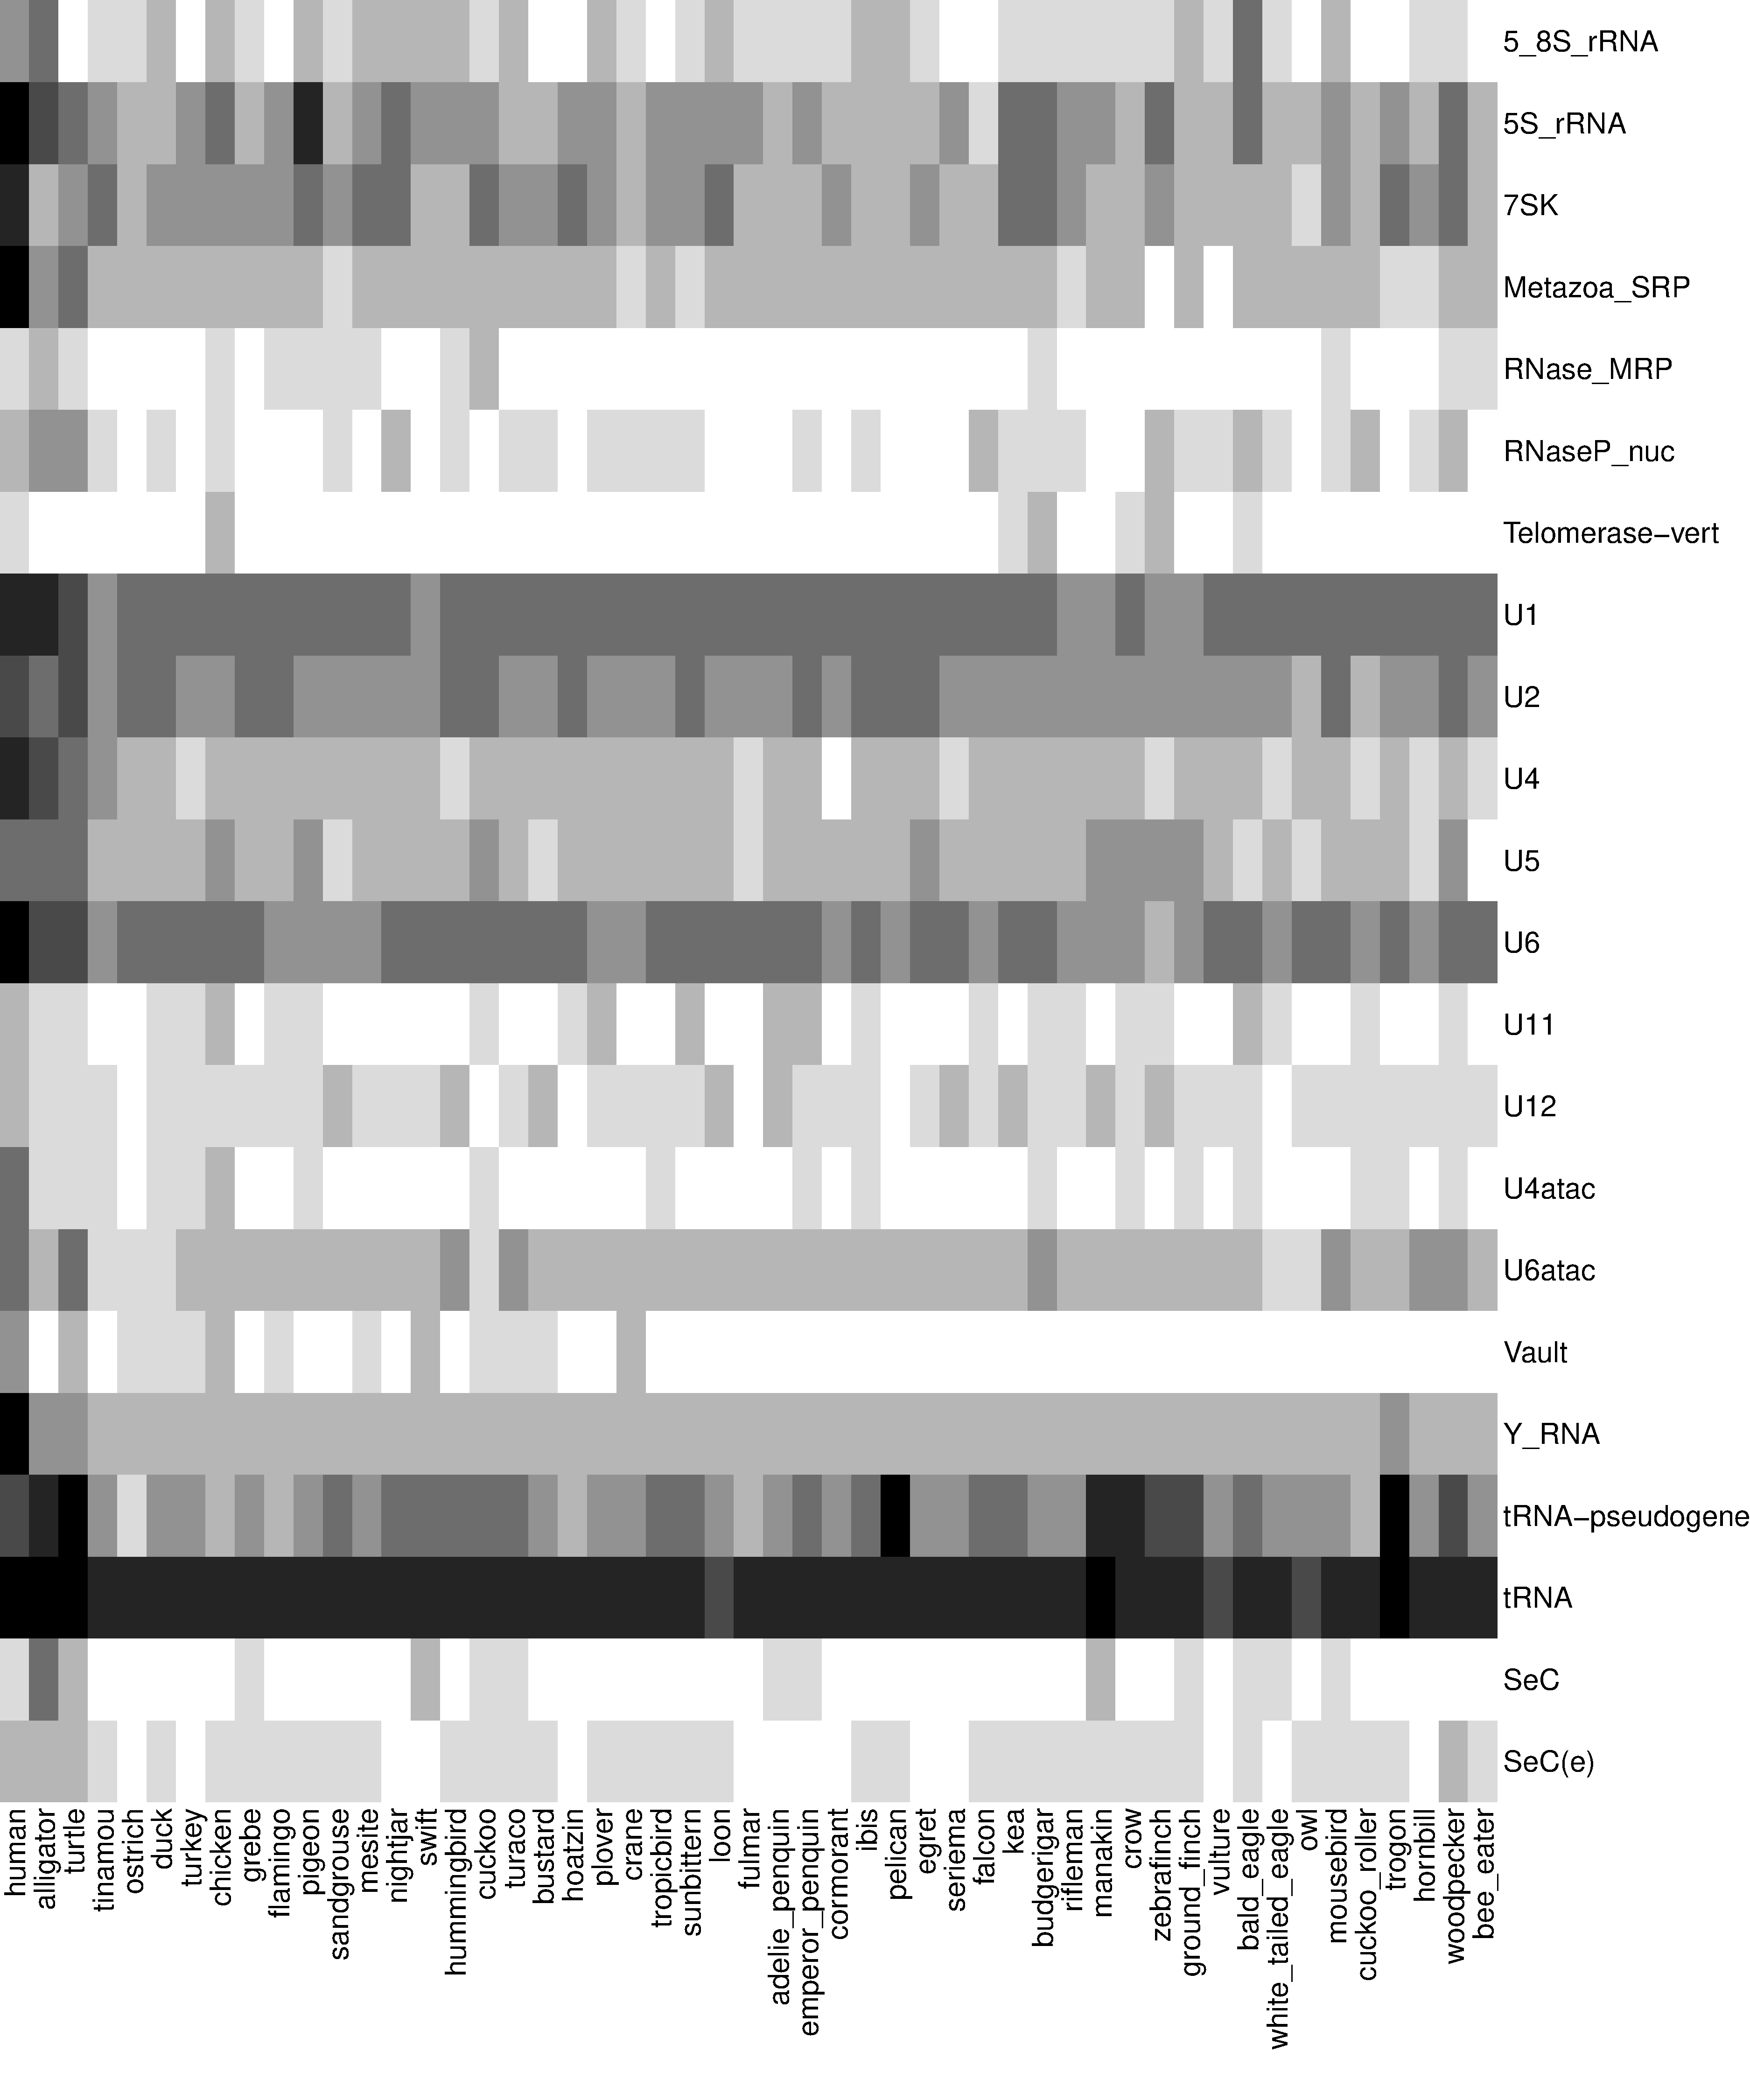
\includegraphics[width=0.45\textwidth]{figures/diverged.pdf}
  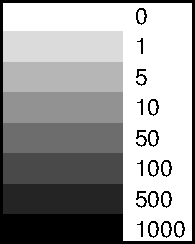
\includegraphics[width=0.1\textwidth]{figures/key2.pdf}
  \caption[]{Heatmaps showing the prescence/abscence and approximate
    genomic copy number of ``unusually, well conserved RNAs''
    (particularly the lncRNAs) on the left and families that have been
    identified as surprising RNA Losses, divergence or missing
    data. In several cases functionally related families have also
    been included, e.g. the RNA components of the major and minor
    spliceosomes: U1, U2, U4, U5 and U6; and U11, U12, U4atac, U5 and
    U6atac, respectively.}\label{fig:5}
\end{figure}


\begin{figure}[ht]
  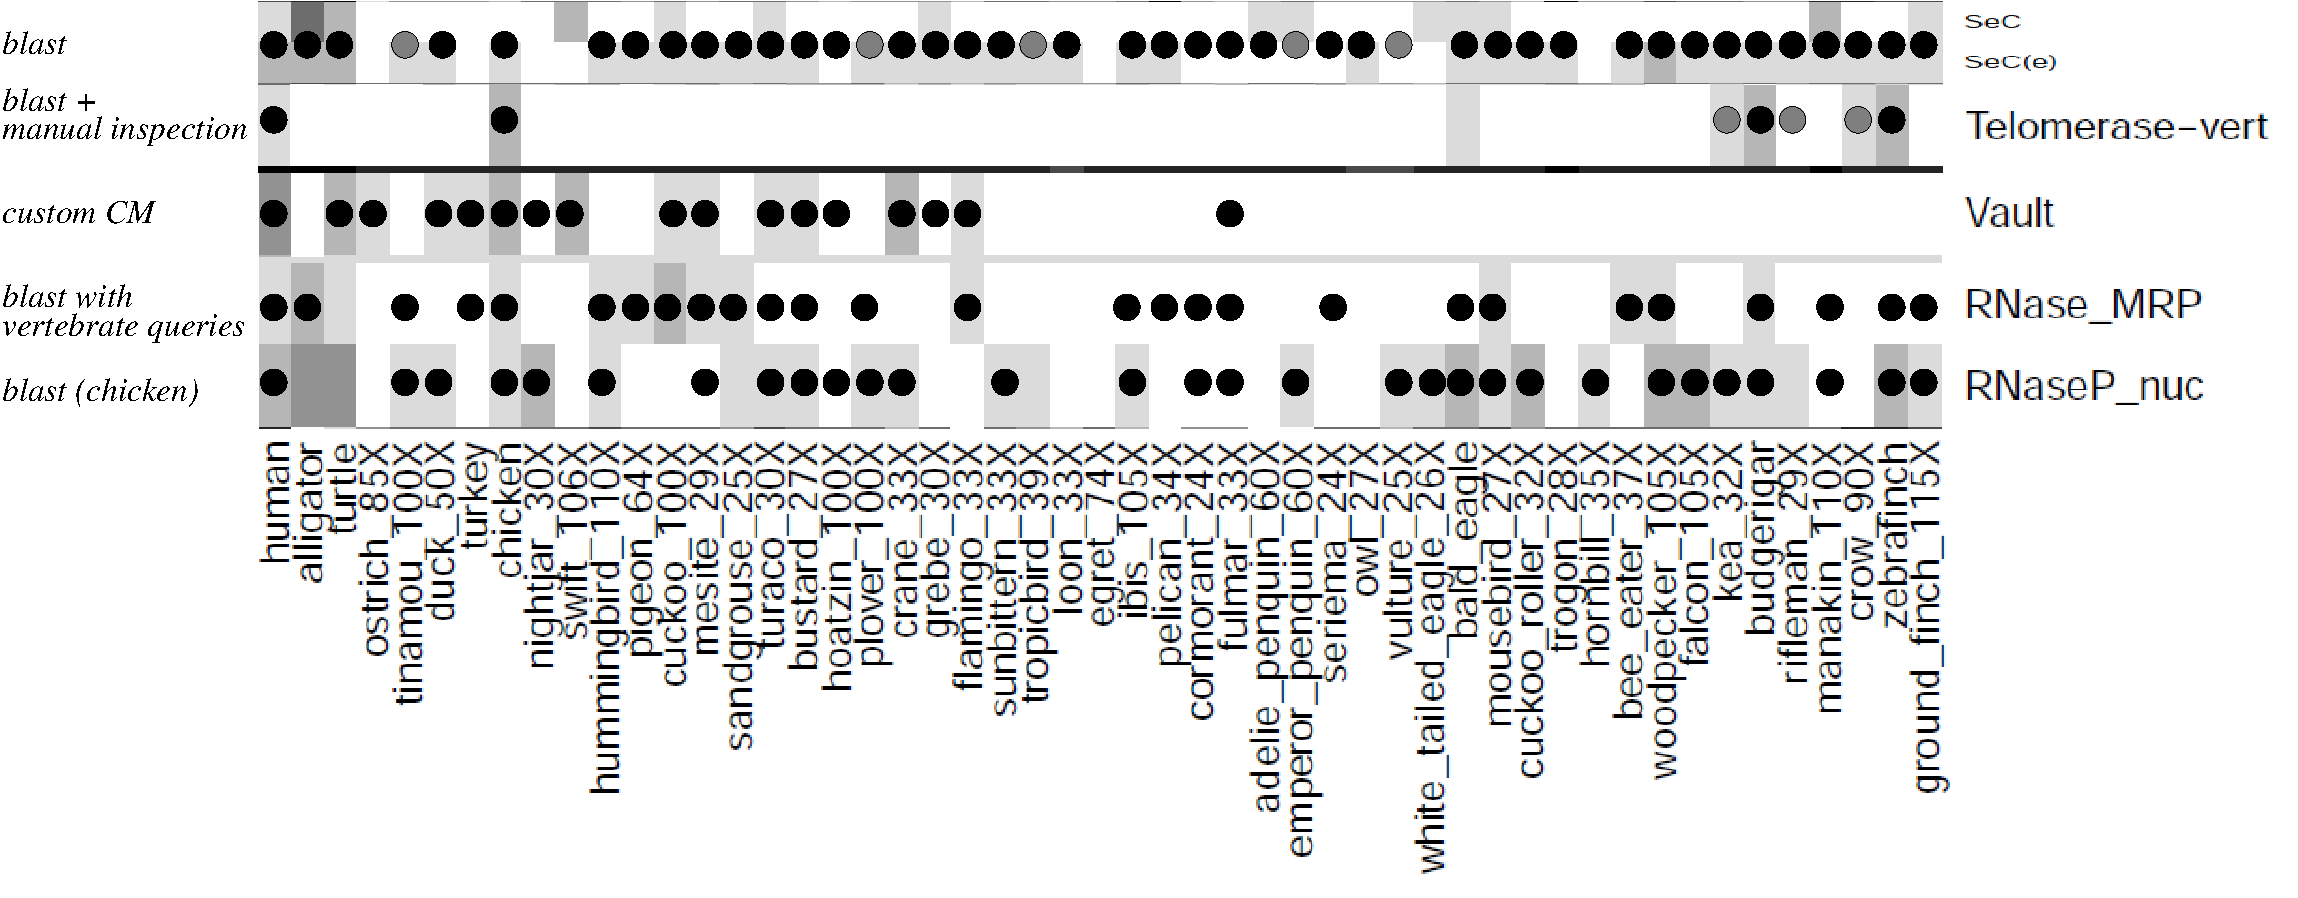
\includegraphics[width=0.75\textwidth]{figures/More-cand.pdf}
  \caption[]{Additional homologs of some sparsely represented RNA
    families were discovered using dedicated search strategies
    combined with highly sensitive settings, synteny information,
    lineage-specific CMs and subsequent manual
    inspection.}\label{fig:7}
\end{figure}





\end{bmcformat}
\end{document}

%%% Local Variables:
%%% mode: latex
%%% TeX-master: t
%%% End: 
